% -*- TeX -*- -*- UK -*- -*- Soft -*-

\chapter{Activation Functions}
\label{sec:ActivationFunctions}

Prepared by CJ Willers.



Several nonlinear functions are used in neural nets, including the sigmoid (logistics), tansig, or soft max
functions\cite{Pedamonti2018,Nwankpa2018,stackexchangeEllefsen2015,WikiPediaHyperbolicfunction2019,NickBecker2017,DustinStansbury2014,HamzaMahmood2018}. 

\section{Linear}

A linear function simply passes the signal with no change or compression
\begin{equation}
g(x)=kx.
\end{equation}  
The derivative of the linear function is the slope of the linear function
\begin{equation}
g^\prime(x) = k
\end{equation}
This function is linear and unbounded. The function is strictly increasing or decreasing (depending on the value of $k$). The function has little application except in cases where the linear output is specifically required.


\section{Logistic Sigmoid}

The sigmoid or logistics function is defined as (see Figure~\ref{fig:sigmoid}):
\begin{equation}
\sigma(x)
=\frac{1}{1+e^{-x}}.
\end{equation}  
The derivative of the sigmoid function is 
\begin{equation}
 \sigma^\prime(x)
 =\sigma(x)(1-\sigma(x))
\end{equation}
The notation $\textrm{sigm}()$ is sometimes used.
This function compresses the output bounded between 0 and 1, is always positive. The function is strictly increasing. Some recent research consider the logistic sigmoid function 'old-fashioned' and limited in value.

\begin{figure}[p]
\centering
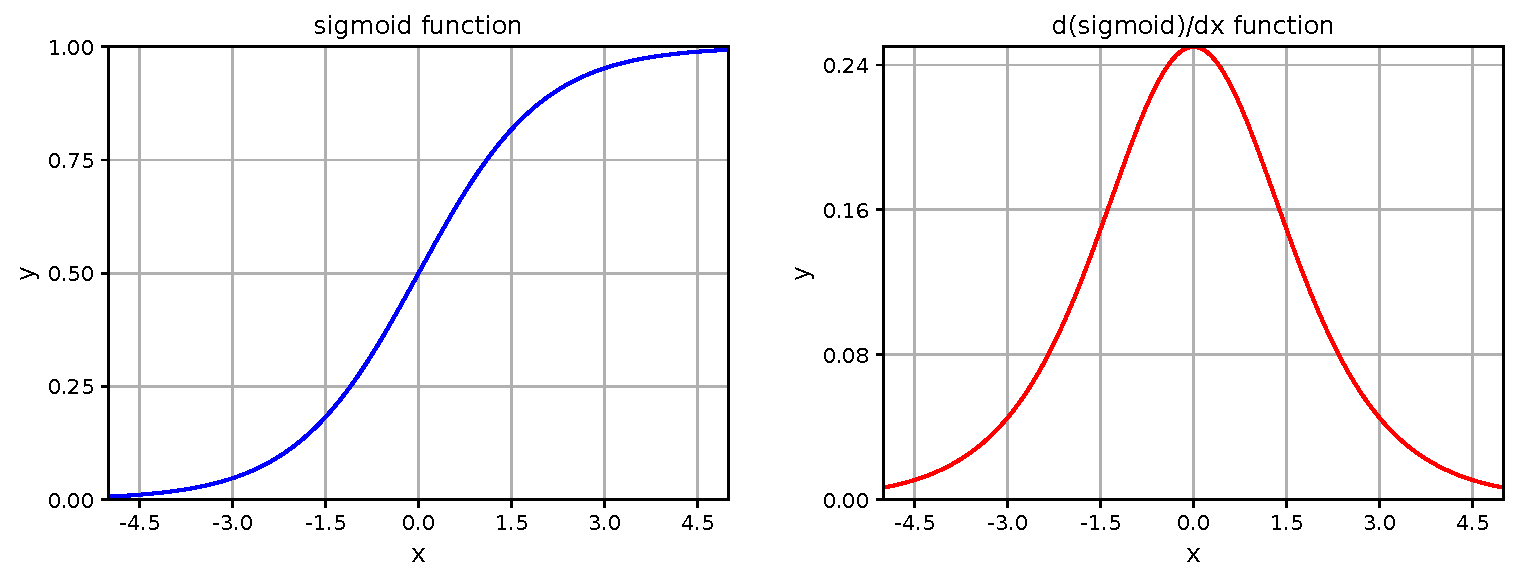
\includegraphics[width=\textwidth]{pic/sigmoid01}
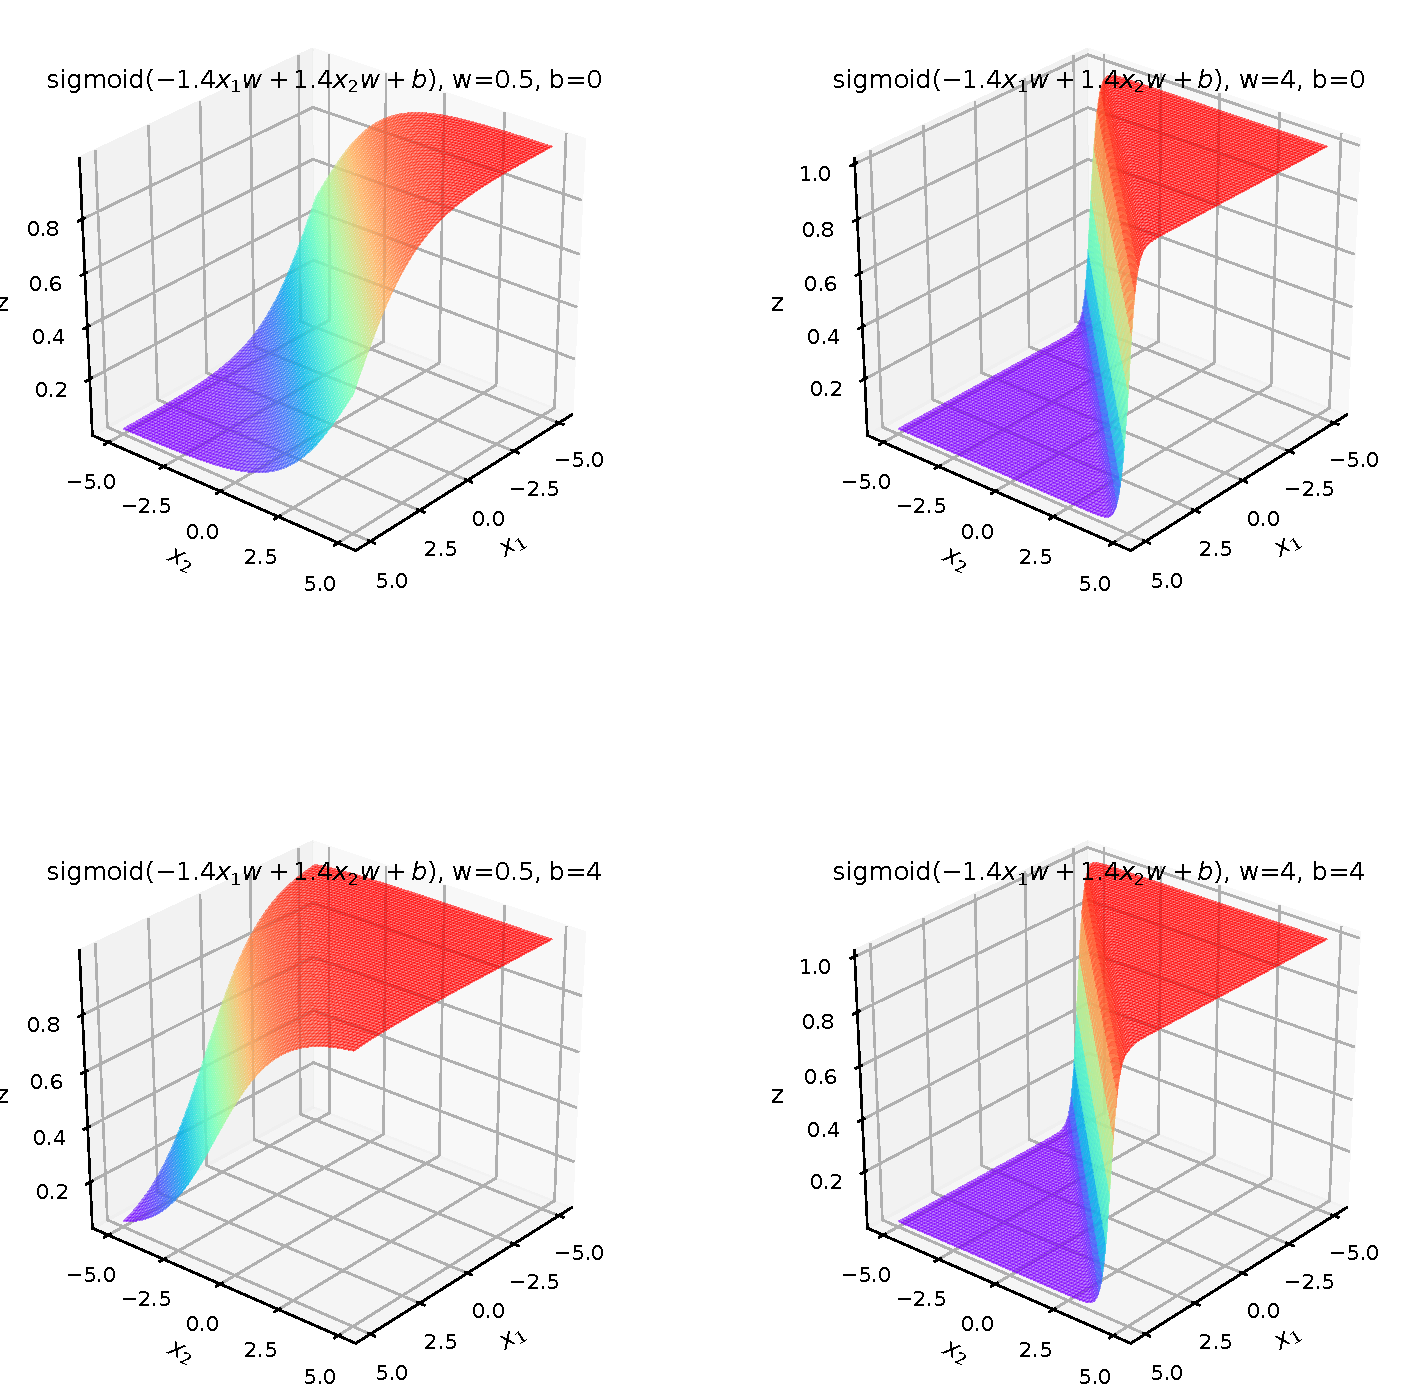
\includegraphics[width=\textwidth]{pic/sigmoid02}
\caption{The sigmoid function }
\label{fig:sigmoid}
\end{figure}


\section{Tansig or tanh}

The tansig function is defined as (see Figure~\ref{fig:tansig}):
\begin{equation}
\textrm{tanh}(x)
=\left(\frac{e^{x}-e^{-x}}{e^{x}+e^{-x}}\right)
=\left(\frac{e^{2x}-1}{e^{2x}+1}\right)
=\left(\frac{1-e^{-2x}}{1+e^{-2x}}\right)
=\left(\frac{2}{1+e^{-2x}}\right)-1,
\end{equation}  
but it is also sometimes seen in a (non-tanh) form:
\begin{equation}
\varphi(x)
=\left(\frac{1-e^{-bx}}{1+e^{-bx}}\right)
=\left(\frac{e^{bx}-1}{e^{bx}+1}\right)
=\left(\frac{2}{1+e^{-bx}}\right)-1
\end{equation}  
where, if $b=2$ yields the $\tanh(x)$ function.
The derivative of the tansig function is 
\begin{equation}
 \varphi^\prime(x)
 = \frac{b}{2} \left(1+\varphi(x))(1-\varphi(x)\right)
 = \frac{b}{2}\left(1-\varphi^2(x)\right)
\end{equation}
The notation $\textrm{tanh}()$ is sometimes used.
This function compresses the output bounded between -1 and 1. The function is strictly increasing. 



\begin{figure}[p]
\centering
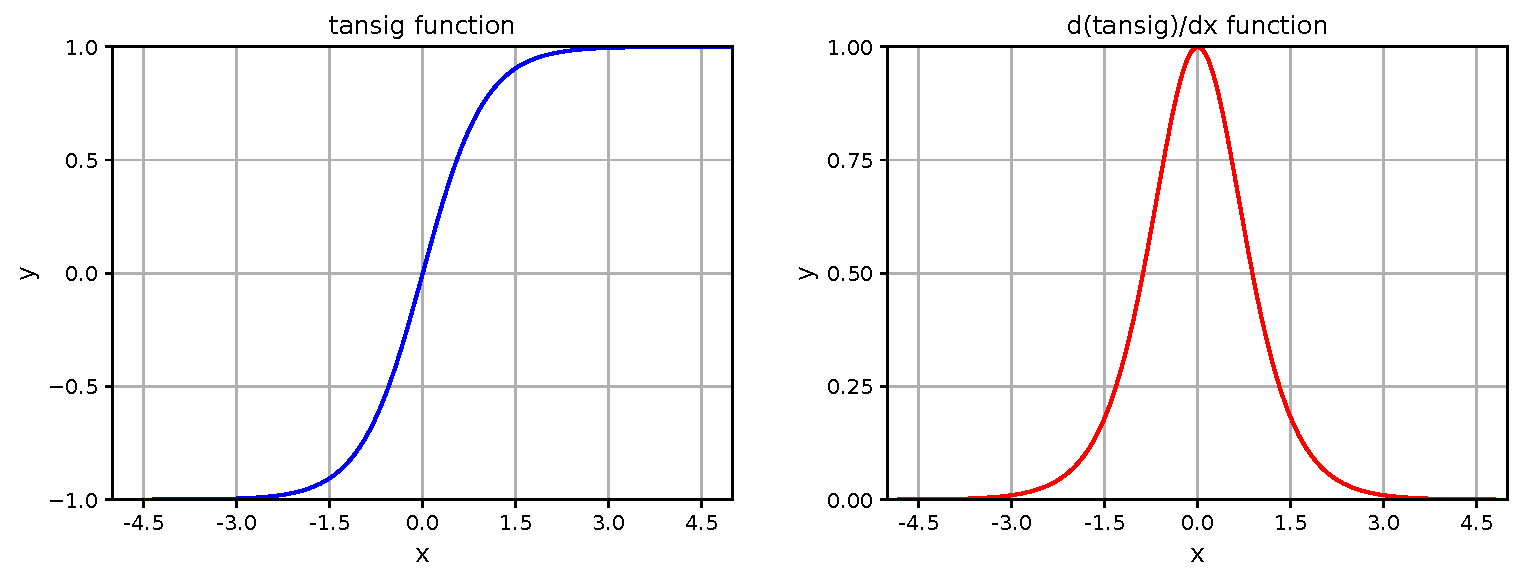
\includegraphics[width=\textwidth]{pic/tansig01}
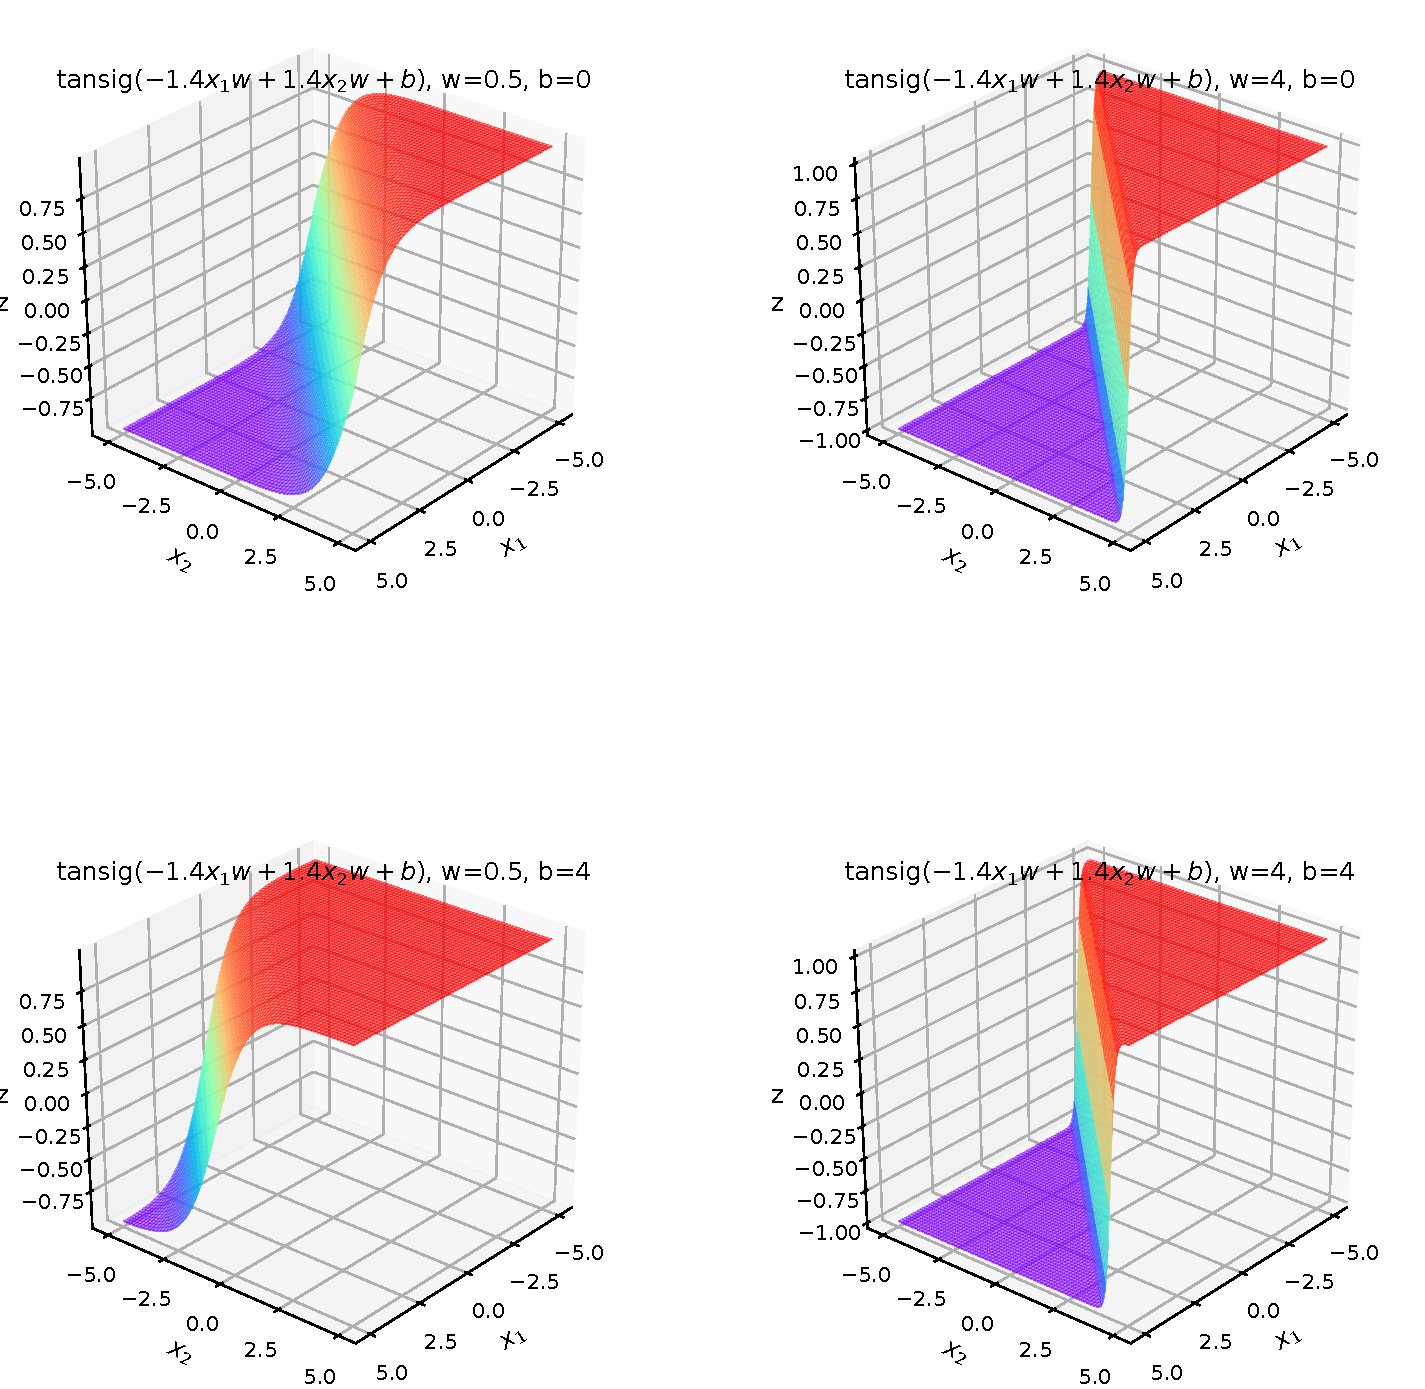
\includegraphics[width=\textwidth]{pic/tansig02}
\caption{The tansig function }
\label{fig:tansig}
\end{figure}



\section{Rectified Linear or reclin}

The reclin function is defined as 
\begin{equation}
\textrm{reclin}(x) = \textrm{max}(0,kx)
\end{equation}
The reclin function is bounded below by 0, it is always non-negative, but has no upper bound.  This function tends to result in neurons with sparse activity, in this case 0 output for all negative inputs.


\TBC{todo}
\begin{lstlisting}

https://en.wikipedia.org/wiki/Softmax_function

https://towardsdatascience.com/softmax-function-simplified-714068bf8156

https://theclevermachine.wordpress.com/2014/09/08/derivation-derivatives-for-common-neural-network-activation-functions/

https://towardsdatascience.com/interpretable-neural-networks-45ac8aa91411

https://stats.stackexchange.com/questions/48470/interpreting-the-output-of-a-neural-network

https://dsotb.quora.com/Deep-learning-with-Keras-convolutional-neural-networks-demystified
\end{lstlisting} 